\documentclass[hide notes]{beamer}
%\documentclass[only notes]{beamer}
\usepackage[english]{babel}
\usepackage{microtype}
\usepackage{environ}
\usepackage{amsmath}
\usepackage[backend=bibtex,style=phys]{biblatex}
\usepackage{doi}
\usepackage{graphicx}
\usepackage{rotating}
\usepackage{tabularx}
\usepackage{dcolumn}
\usepackage{booktabs}
\usepackage{scrextend} % for \footref
\usepackage{hyperref}
\usepackage[nameinlink,capitalize]{cleveref}
\usepackage{siunitx}
\usepackage{floatrow}
\usepackage{bm}
\usepackage{mathtools}

% style stuff
\usetheme{osu}
\hypersetup{hidelinks}
\bibliography{thesis.bib}
% http://tex.stackexchange.com/questions/21913/how-can-i-change-the-footnote-line-thickness-length
\renewcommand{\footnoterule}{%
  \kern -3pt
  \hrule width \textwidth height 0.5pt
  \kern 2pt
}
% http://tex.stackexchange.com/questions/21741/how-do-i-change-footnote-font-size-in-beamer-presentation
\let\oldfootnotesize\footnotesize
\renewcommand*{\footnotesize}{\oldfootnotesize\tiny}
% http://tex.stackexchange.com/questions/169745/left-aligning-footnotes-in-beamer
\makeatletter
\renewcommand<>\beamer@framefootnotetext[1]{%
  \global\setbox\beamer@footins\vbox{%
    \hsize\framewidth
    \textwidth\hsize
    \columnwidth\hsize
    \unvbox\beamer@footins
    \reset@font\footnotesize
    \@parboxrestore
    \protected@edef\@currentlabel
         {\csname p@footnote\endcsname\@thefnmark}%
    \color@begingroup
      \uncover#2{\@makefntext{%
        \rule\z@\footnotesep\ignorespaces\parbox[t]{.9\textwidth}{#1\@finalstrut\strutbox}\vskip1sp}}%
    \color@endgroup}%
}
\makeatother

% custom commands
\DeclareMathOperator{\Tanh}{\mathbf{tanh}}
\DeclarePairedDelimiter\ceil{\lceil}{\rceil}
\DeclarePairedDelimiter\floor{\lfloor}{\rfloor}
% footnote without marker
% https://tex.stackexchange.com/questions/30720/footnote-without-a-marker
\newcommand\blfootnote[1]{%
  \begingroup
  \renewcommand\thefootnote{}\footnote{#1}%
  \addtocounter{footnote}{-1}%
  \endgroup
}
% toc slide
\newcommand\tocframe{%
  \frame{\tableofcontents[currentsection,hideallsubsections]}
}

% use dcolumn
\newcolumntype{d}{D{.}{.}{-1}}
\newcolumntype{e}{D{.}{.}{8}}
\newcolumntype{f}{D{.}{.}{13}}

\title{Essential Reservoir Computing}
%\subtitle{}

\author[Griffith]{Aaron Griffith}
\institute[Ohio State University]{Department of Physics\\Ohio State University}
\date[8/17/2021]{August 17, 2021}

\begin{document}

\begin{frame}[plain]
  \titlepage
\end{frame}

%\setbeamertemplate{footline}[frame number]{\tiny\insertframenumber\,/\,\inserttotalframenumber}
% https://tex.stackexchange.com/questions/434923/frame-number-does-not-work-since-ubuntu-update?noredirect=1&lq=1
\setbeamertemplate{navigation symbols}{\textcolor{osured}{\tiny\insertframenumber\,/\,\inserttotalframenumber}}

\section{Introduction}

\frame{\tableofcontents[hideallsubsections]}

\begin{frame}{Machine Learning and Neural Networks}
  \begin{columns}
    \column{0.5\textwidth}
    \begin{itemize}
    \item neural networks are universal models
    \item learn relationship between input and output from example data
    \item very useful if this relationship is unknown, but examples are easy to find
    \item canonical example: learn how to turn images of digits into labels
    \end{itemize}
    \column{0.5\textwidth}
    \centering
    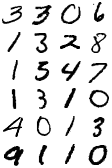
\includegraphics[width=0.7\textwidth]{figures/mnist.png}
  \end{columns}
\end{frame}

\begin{frame}{Machine Learning in Physics}
  \begin{itemize}
  \item Elsewhere:
    \begin{itemize}
    \item find masses of particles from decay data\footnote{\fullcite{lonnblad1992}}
    \item separate quark and gluon jets in $e^+ e^-$ annihilation\footnote{\fullcite{csabai1991}}
    \end{itemize}
  \item In this presentation:
    \begin{itemize}
    \item \textbf{system state inference}: given $x(t)$ and $y(t)$, find $z(t)$
    \item \textbf{chaotic system forecasting}: given the beginning of a signal $u(t)$, what happens after?
    \end{itemize}
  \end{itemize}
\end{frame}

\begin{frame}{Chaotic System Forecasting}
  \centering
  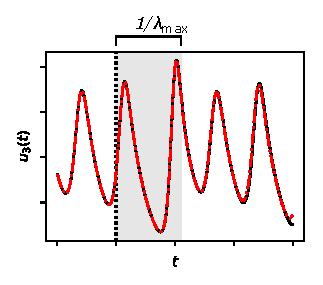
\includegraphics[width=0.7\textwidth]{figures/prediction-example.eps}
\end{frame}

\begin{frame}{The Problem with Neural Networks}
  \begin{itemize}
  \item very expensive to train
    \begin{itemize}
    \item data hungry: require many examples
    \item deep networks take longer to train: ``vanishing gradient problem''
    \end{itemize}
  \item alternative: \textbf{Reservoir Computers}
    \begin{itemize}
    \item quick training
    \item physical interpretation
    \item physical implementation
    \end{itemize}
  \end{itemize}
\end{frame}

\section{Reservoir Computing}

\tocframe

\section{Low-Connectivity Reservoirs}

\tocframe

\section{RCs without Reservoirs: NVARs}

\tocframe

\section{NVARs in Practice}

\tocframe

\section{Conclusion}

\tocframe

\begin{frame}
  \begin{center}
    {\usebeamercolor[fg]{frametitle}{\Large Thank you!}}

    Questions?
  \end{center}

  \note{o7}
\end{frame}

\end{document}

